\subsubsection{Caveats and considerations}
\label{sec:analysis-correlation-results-caveats}

\begin{enumerate}
\item Computing ACF per cell vs per time point
\label{sec:org8575590}

Insert content here

\item Non-stationary envelope function can be ignored
\label{sec:org638bcff}

\begin{enumerate}
\item Approach
\label{sec:org68672a6}

Let \(f(t) = K_{\rm{min}} + K_{\rm{max}}(1 - \rm{e}^{-t/\tau})\) (a logistic function), a simple example of a function that makes a process non-stationary.  \(K_{\rm{min}}\) is there to make the amplitude of the oscillation never zero.

Define the oscillatory function as \(y(t) = f(t)sin(\omega{}t + \phi)\) as a simple example, i.e. \(f(t)\) replaces the amplitude of the sinusoid -- implies that the amplitude changes depending on time.

Add white noise.

\item Results
\label{sec:org7f403a8}

I defined the underlying function as \(f(t)\) and the oscillatory function as \(y(t)\), as above.  Then added white noise (standard deviation = 1).

\begin{enumerate}
\item Same phase
\label{sec:org0e46814}

First, I set each oscillatory function to start at the same phase (i.e. \(\phi = 0\)).

For the underlying function, I set \(K_{\rm{min}} = 1\), \(K_{\rm{max}} = 10\), \(\tau = 100\):
\begin{center}
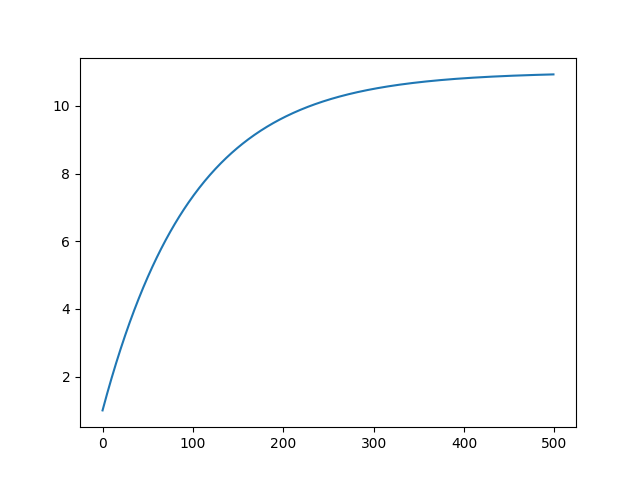
\includegraphics[width=.9\linewidth]{envelope_function_kmax10.png}
\end{center}

When I generated 3 replicates:
\begin{center}
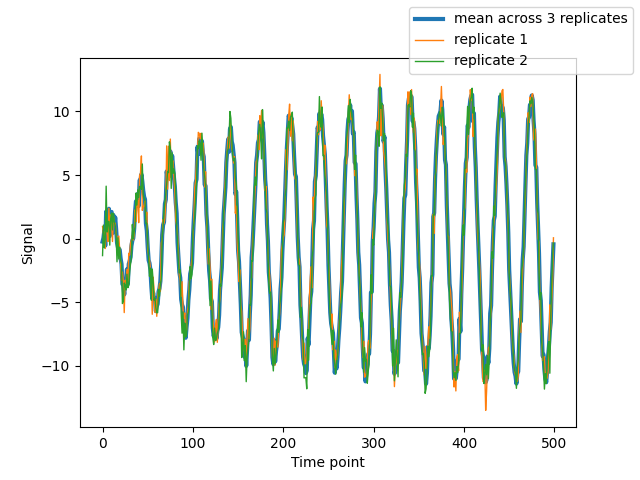
\includegraphics[width=.9\linewidth]{nonstat_kmax10_samephase_3rep_mean.png}
\end{center}
\begin{center}
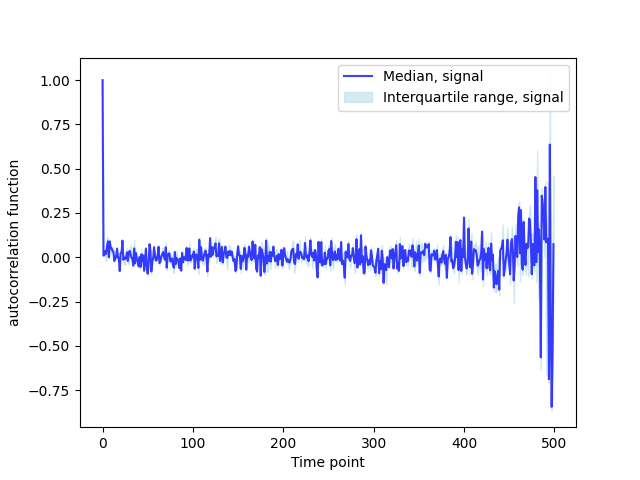
\includegraphics[width=.9\linewidth]{nonstat_kmax10_samephase_3rep_acf.png}
\end{center}

Changing the underlying function (\(K_{\rm{max}} = 1000\)) still produced a similar autocorrelation function, but differed from the previous due to noise:
\begin{center}
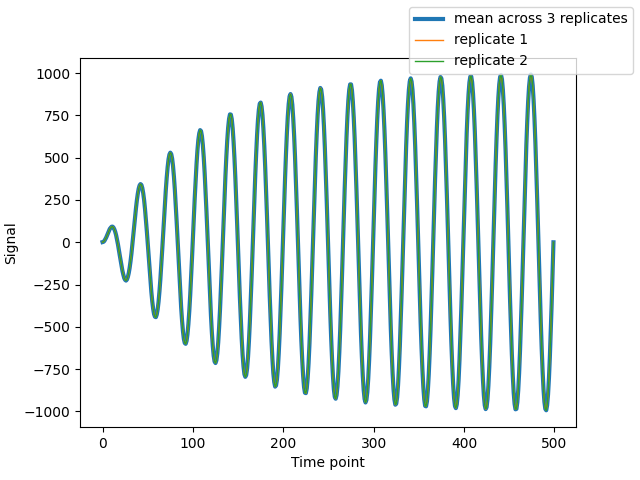
\includegraphics[width=.9\linewidth]{nonstat_kmax1000_samephase_3rep_mean.png}
\end{center}
\begin{center}
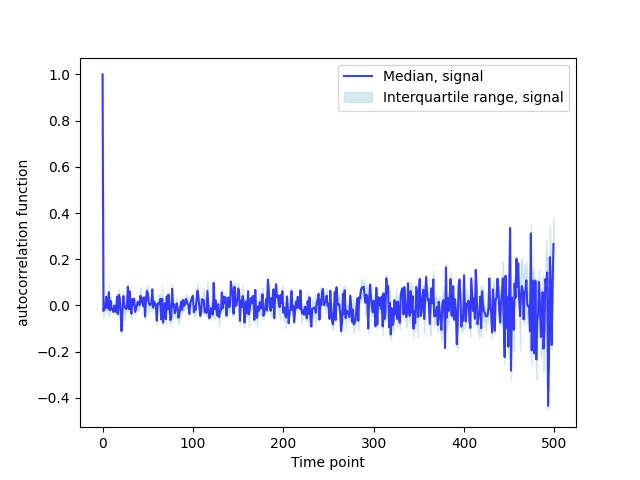
\includegraphics[width=.9\linewidth]{nonstat_kmax1000_samephase_3rep_acf.png}
\end{center}

Increasing the number of replicates to 1000 smoothed the mean across replicates (not shown here) and reduced the `noise' in the autocorrelation function:

(\(K_{\rm{max}} = 10\))
\begin{center}
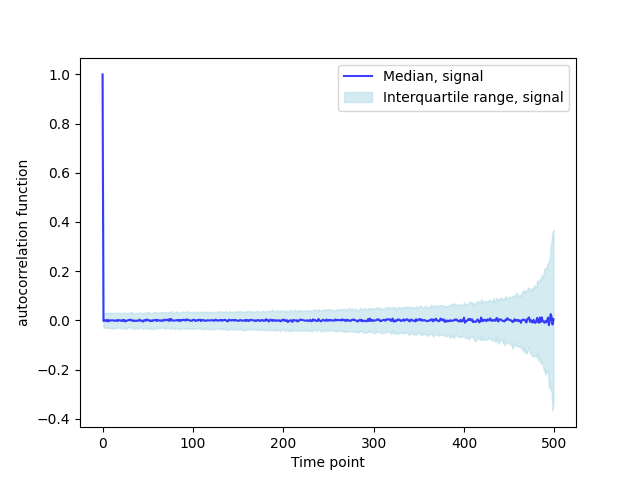
\includegraphics[width=.9\linewidth]{nonstat_kmax10_samephase_1000rep_acf.png}
\end{center}

(\(K_{\rm{max}} = 1000\))
\begin{center}
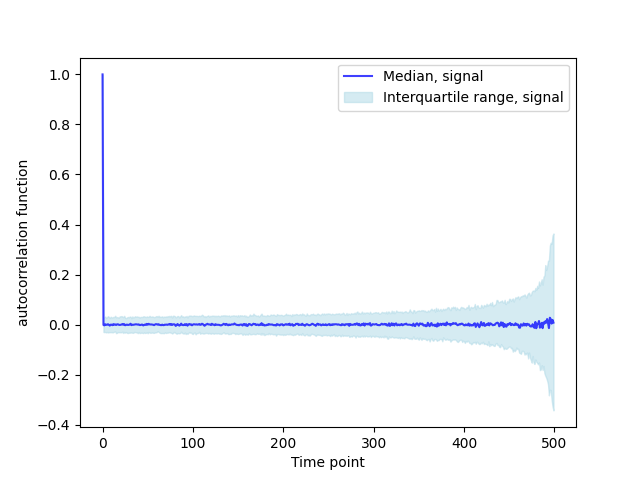
\includegraphics[width=.9\linewidth]{nonstat_kmax1000_samephase_1000rep_acf.png}
\end{center}

(\(\tau = 1000, K_{\rm{max}} = 10\))
\begin{center}
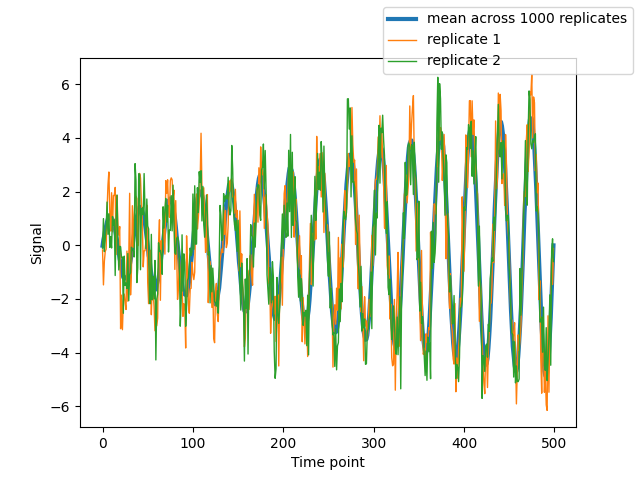
\includegraphics[width=.9\linewidth]{nonstat_tau1000_samephase_1000rep_mean.png}
\end{center}
\begin{center}
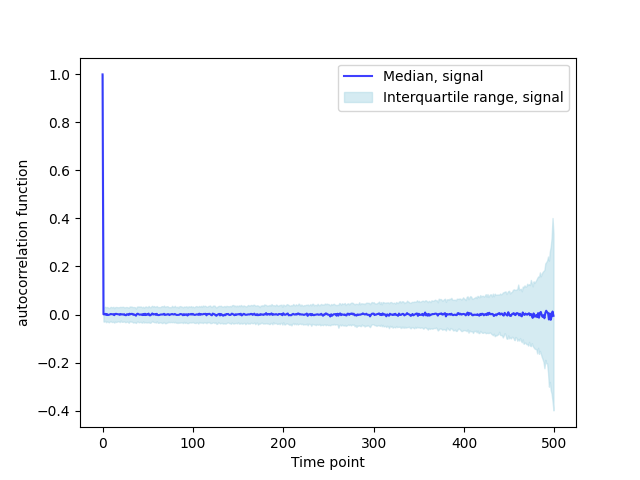
\includegraphics[width=.9\linewidth]{nonstat_tau1000_samephase_1000rep_acf.png}
\end{center}

The variation in autocorrelation functions near the right end does not seem to be a function of noise.  Here is with \(\sigma = 5\) for the Gaussian distribution the white noise is derived from (\(K_{\rm{max}} = 10\)):
\begin{center}
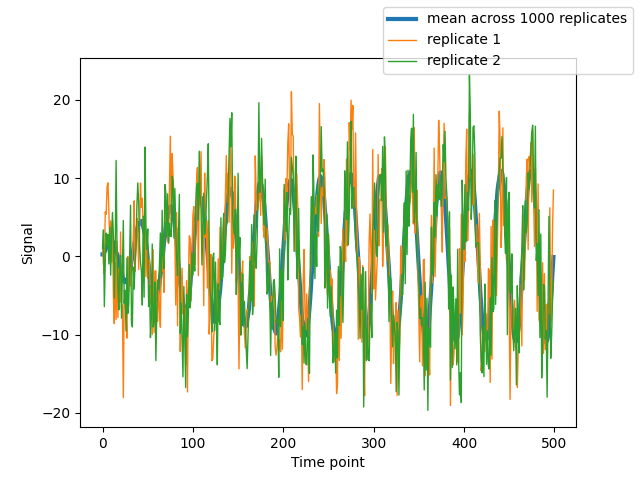
\includegraphics[width=.9\linewidth]{nonstat_kmax10_samephase_1000rep_mean_noisier.png}
\end{center}
\begin{center}
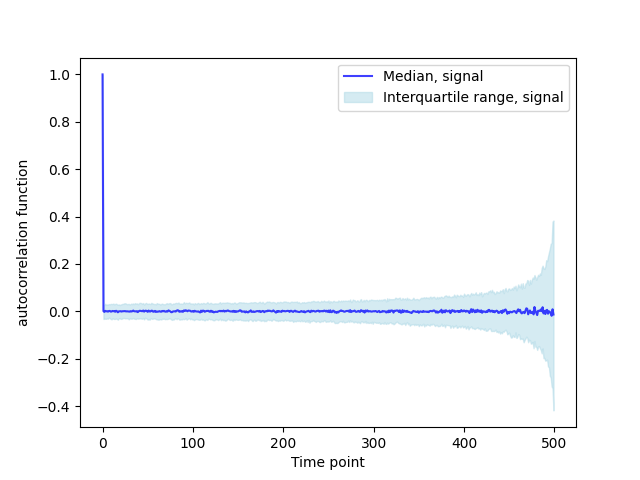
\includegraphics[width=.9\linewidth]{nonstat_kmax10_samephase_1000rep_acf_noisier.png}
\end{center}


\item Random phases
\label{sec:orgd672617}

Next, I set each oscillatory function to start at a random phase between 0 and 2\(\pi\).

When I generated 3 replicates (\(K_{\rm{max}} = 10, \sigma = 1\)), the mean across replicates has a relatively high amplitude.  The autocorrelation function was smooth but showed damping:
\begin{center}
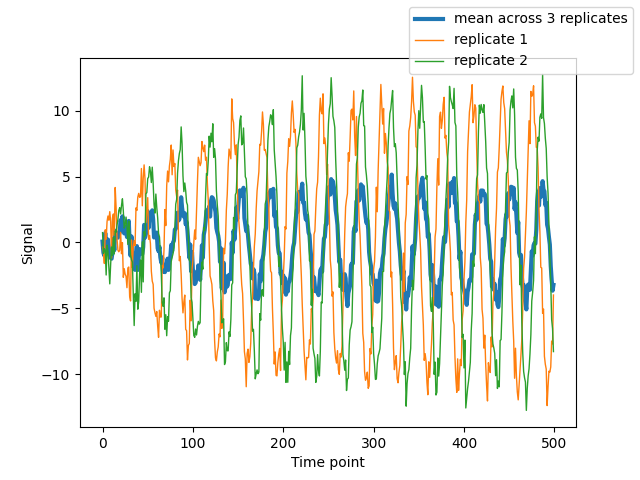
\includegraphics[width=.9\linewidth]{nonstat_kmax10_randphase_3rep_mean.png}
\end{center}
\begin{center}
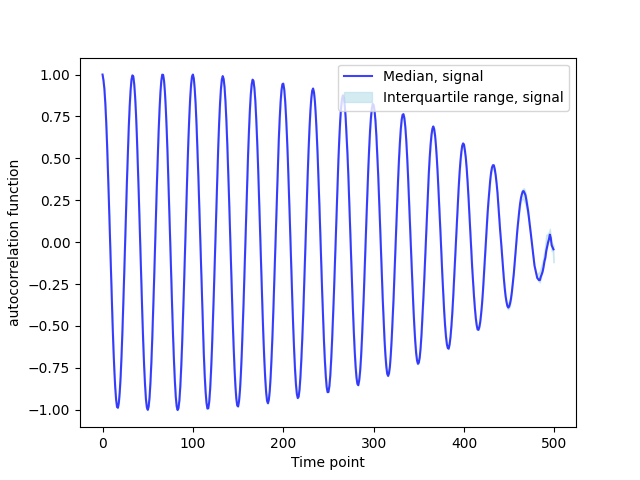
\includegraphics[width=.9\linewidth]{nonstat_kmax10_randphase_3rep_acf.png}
\end{center}

Increasing the number of replicates to 1000 decreased the amplitude of the mean across replicates, likely because there are more out-of-phase signals to cancel each other out.  The autocorrelation function is largely unchanged, save for the slight increase in variability as the lag approaches the length of the time series (blue: 3 replicates, red: 1000 replicates):
\begin{center}
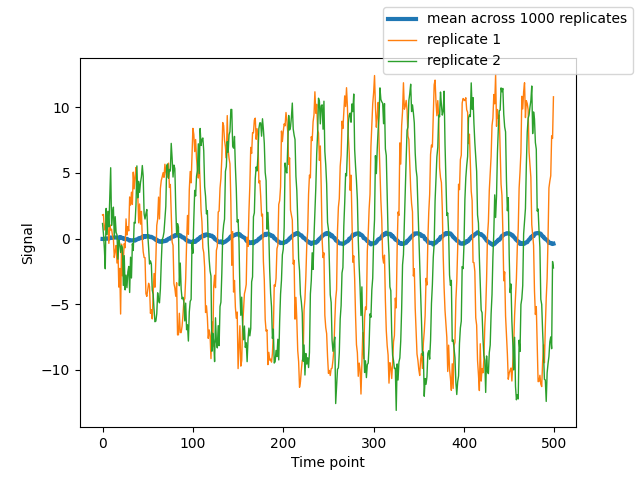
\includegraphics[width=.9\linewidth]{nonstat_kmax10_randphase_1000rep_mean.png}
\end{center}

\begin{center}
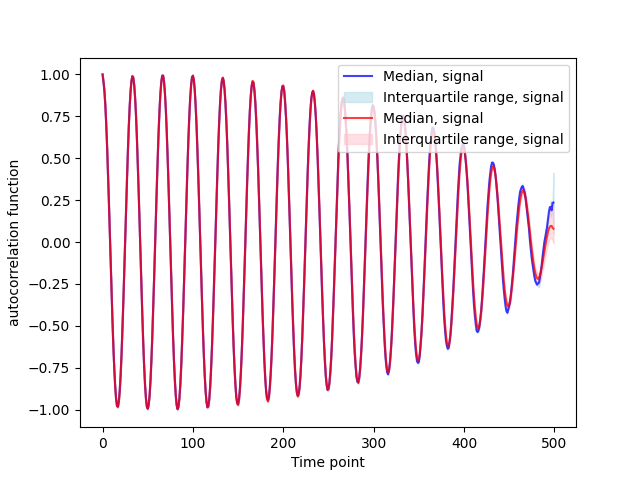
\includegraphics[width=.9\linewidth]{nonstat_3vs1000rep.png}
\end{center}
\begin{center}
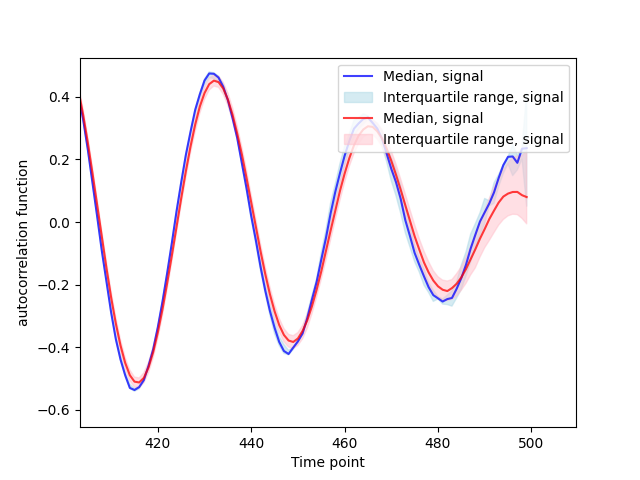
\includegraphics[width=.9\linewidth]{nonstat_3vs1000rep_zoom.png}
\end{center}

Comparing 3 replicates and 1000 replicates, the autocorrelation functions are more similar at smaller lags.

With fewer data points (75 instead of 500) and therefore less information, the autocorrelation function from 3 replicates and from 1000 replicates diverge more.  In other words, it is clear that the quality of the autocorrelation function from 3 replicates is lower:
\begin{center}
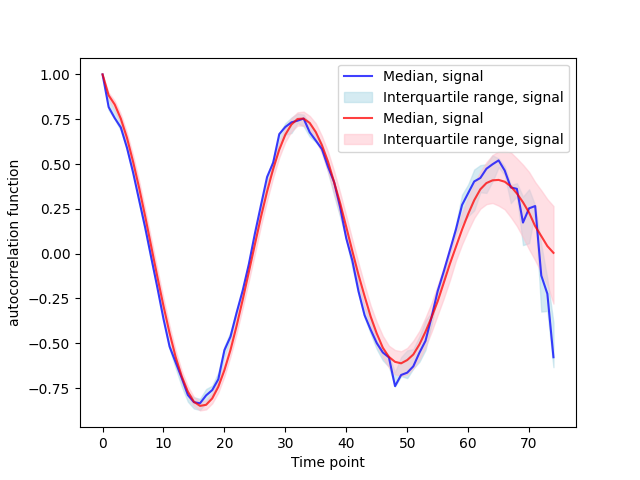
\includegraphics[width=.9\linewidth]{nonstat_3vs1000rep_shorter.png}
\end{center}

This effect is strengthened when there is more noise (\(\sigma = 5\)).  Also note the larger interquartile range as lag increases for the 1000-replicate autocorrelation function:
\begin{center}
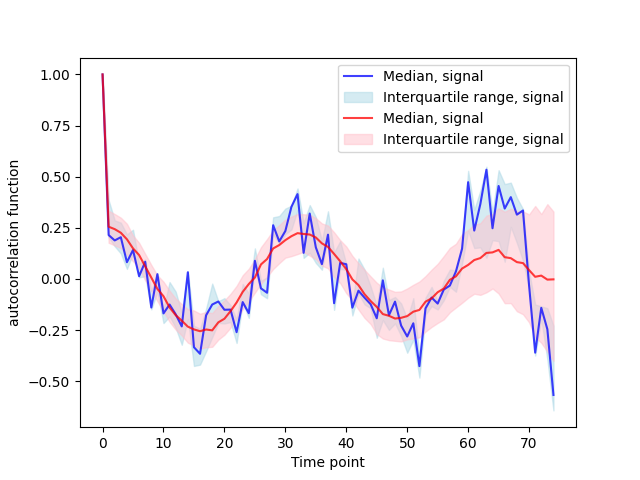
\includegraphics[width=.9\linewidth]{nonstat_3vs1000rep_shorter_noisier.png}
\end{center}

\begin{enumerate}
\item Effect of underlying function
\label{sec:orgb7bbe3a}

Changing the underlying function changes the autocorrelation function, even if there are 1000 replicates.

(blue: \(K_{\rm{max}} = 10\), red: \(K_{\rm{max}} = 1000\)):
\begin{center}
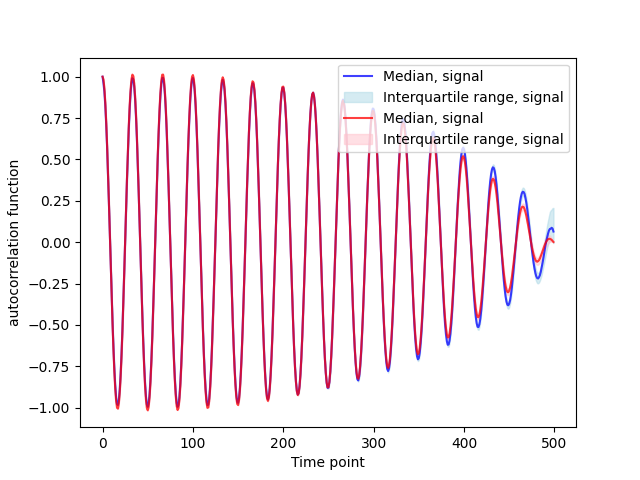
\includegraphics[width=.9\linewidth]{nonstat_kmax_effect.png}
\end{center}

(blue: \(\tau = 100\), red: \(\tau = 1000\)):
\begin{center}
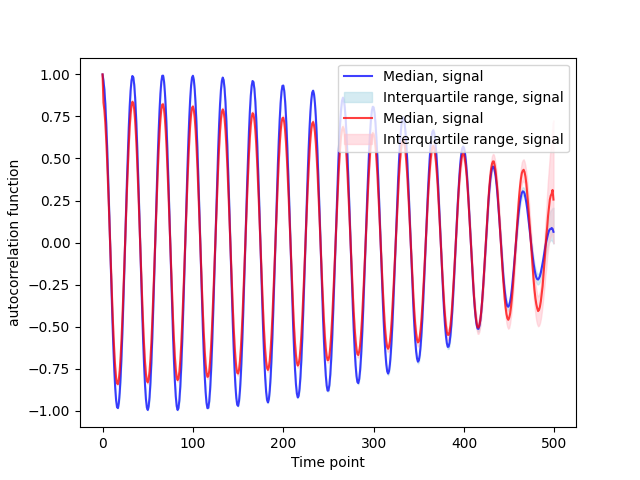
\includegraphics[width=.9\linewidth]{nonstat_tau_effect.png}
\end{center}

The effect is the same if there are 3 replicates.
\end{enumerate}
\end{enumerate}

\item Conclusions
\label{sec:org5312d3c}

The underlying function does not affect the autocorrelation function if all signals are in-phase -- this makes sense given that the underlying function is subtracted from all signals when the autocorrelation is computed, leaving behind just noise.  In contrast, if the signals are not in-phase, the underlying function affects the autocorrelation function, particularly if there are many replicates.  This makes sense as the phases cancel out when the mean across replicates is computed, and the underlying function component of each time series remains.

As the number of replicates increases, the shape of the autocorrelation function changes until it converges towards an `ideal' function.  This is likely because there is more information to accurately estimate the mean -- changes to the number of time points and the noise which reduce information content seem to support this idea.  More information is needed to estimate longer lags because the number of data points used to calculate the autocorrelation decreases with lag, as per the definition of cross-correlation:

\begin{equation}
c_{k} = \sum_{n} a_{n+k} \cdot \overline{v_n}
\end{equation}

where \(a\) and \(v\) are the two time series to be correlated, and \(\overline{x}\) denotes complex conjugation.
\end{enumerate}
\end{enumerate}
